% Options for packages loaded elsewhere
\PassOptionsToPackage{unicode}{hyperref}
\PassOptionsToPackage{hyphens}{url}
%
\documentclass[
  11pt,
  ignorenonframetext,
  aspectratio=169,
  c]{beamer}
\usepackage{pgfpages}
\setbeamertemplate{caption}[numbered]
\setbeamertemplate{caption label separator}{: }
\setbeamercolor{caption name}{fg=normal text.fg}
\beamertemplatenavigationsymbolshorizontal
% Prevent slide breaks in the middle of a paragraph
\widowpenalties 1 10000
\raggedbottom
\setbeamertemplate{part page}{
  \centering
  \begin{beamercolorbox}[sep=16pt,center]{part title}
    \usebeamerfont{part title}\insertpart\par
  \end{beamercolorbox}
}
\setbeamertemplate{section page}{
  \centering
  \begin{beamercolorbox}[sep=12pt,center]{part title}
    \usebeamerfont{section title}\insertsection\par
  \end{beamercolorbox}
}
\setbeamertemplate{subsection page}{
  \centering
  \begin{beamercolorbox}[sep=8pt,center]{part title}
    \usebeamerfont{subsection title}\insertsubsection\par
  \end{beamercolorbox}
}
\AtBeginPart{
  \frame{\partpage}
}
\AtBeginSection{
  \ifbibliography
  \else
    \frame{\sectionpage}
  \fi
}
\AtBeginSubsection{
  \frame{\subsectionpage}
}

\usepackage{amsmath,amssymb}
\usepackage{lmodern}
\usepackage{iftex}
\ifPDFTeX
  \usepackage[T1]{fontenc}
  \usepackage[utf8]{inputenc}
  \usepackage{textcomp} % provide euro and other symbols
\else % if luatex or xetex
  \usepackage{unicode-math}
  \defaultfontfeatures{Scale=MatchLowercase}
  \defaultfontfeatures[\rmfamily]{Ligatures=TeX,Scale=1}
\fi
\usetheme[]{Luebeck}
\usecolortheme{beaver}
% Use upquote if available, for straight quotes in verbatim environments
\IfFileExists{upquote.sty}{\usepackage{upquote}}{}
\IfFileExists{microtype.sty}{% use microtype if available
  \usepackage[]{microtype}
  \UseMicrotypeSet[protrusion]{basicmath} % disable protrusion for tt fonts
}{}
\makeatletter
\@ifundefined{KOMAClassName}{% if non-KOMA class
  \IfFileExists{parskip.sty}{%
    \usepackage{parskip}
  }{% else
    \setlength{\parindent}{0pt}
    \setlength{\parskip}{6pt plus 2pt minus 1pt}}
}{% if KOMA class
  \KOMAoptions{parskip=half}}
\makeatother
\usepackage{xcolor}
\newif\ifbibliography
\setlength{\emergencystretch}{3em} % prevent overfull lines
\setcounter{secnumdepth}{-\maxdimen} % remove section numbering


\providecommand{\tightlist}{%
  \setlength{\itemsep}{0pt}\setlength{\parskip}{0pt}}\usepackage{longtable,booktabs,array}
\usepackage{calc} % for calculating minipage widths
\usepackage{caption}
% Make caption package work with longtable
\makeatletter
\def\fnum@table{\tablename~\thetable}
\makeatother
\usepackage{graphicx}
\makeatletter
\def\maxwidth{\ifdim\Gin@nat@width>\linewidth\linewidth\else\Gin@nat@width\fi}
\def\maxheight{\ifdim\Gin@nat@height>\textheight\textheight\else\Gin@nat@height\fi}
\makeatother
% Scale images if necessary, so that they will not overflow the page
% margins by default, and it is still possible to overwrite the defaults
% using explicit options in \includegraphics[width, height, ...]{}
\setkeys{Gin}{width=\maxwidth,height=\maxheight,keepaspectratio}
% Set default figure placement to htbp
\makeatletter
\def\fps@figure{htbp}
\makeatother

\usepackage{tabu}

%\usepackage{emoji}
%\usepackage{xelatexemoji}-
%\AtBeginSection{}
%\renewcommand{\tableofcontents}{...}
%\setbeameroption{show notes}
%\setbeamertemplate{navigation symbols}{}
%\setbeamertemplate{footline}[page number]
        
\usepackage{appendixnumberbeamer}
\usepackage{fontawesome5}
\titlegraphic{
\includegraphics[width=0.6\paperwidth]{Figures/logos/UL-ENSGSI-ERPI.png}}
\makeatletter
\makeatother
\makeatletter
\makeatother
\makeatletter
\@ifpackageloaded{caption}{}{\usepackage{caption}}
\AtBeginDocument{%
\ifdefined\contentsname
  \renewcommand*\contentsname{Table of contents}
\else
  \newcommand\contentsname{Table of contents}
\fi
\ifdefined\listfigurename
  \renewcommand*\listfigurename{List of Figures}
\else
  \newcommand\listfigurename{List of Figures}
\fi
\ifdefined\listtablename
  \renewcommand*\listtablename{List of Tables}
\else
  \newcommand\listtablename{List of Tables}
\fi
\ifdefined\figurename
  \renewcommand*\figurename{Figure}
\else
  \newcommand\figurename{Figure}
\fi
\ifdefined\tablename
  \renewcommand*\tablename{Table}
\else
  \newcommand\tablename{Table}
\fi
}
\@ifpackageloaded{float}{}{\usepackage{float}}
\floatstyle{ruled}
\@ifundefined{c@chapter}{\newfloat{codelisting}{h}{lop}}{\newfloat{codelisting}{h}{lop}[chapter]}
\floatname{codelisting}{Listing}
\newcommand*\listoflistings{\listof{codelisting}{List of Listings}}
\makeatother
\makeatletter
\@ifpackageloaded{caption}{}{\usepackage{caption}}
\@ifpackageloaded{subcaption}{}{\usepackage{subcaption}}
\makeatother
\makeatletter
\@ifpackageloaded{tcolorbox}{}{\usepackage[many]{tcolorbox}}
\makeatother
\makeatletter
\@ifundefined{shadecolor}{\definecolor{shadecolor}{rgb}{.97, .97, .97}}
\makeatother
\makeatletter
\makeatother
\ifLuaTeX
  \usepackage{selnolig}  % disable illegal ligatures
\fi
\IfFileExists{bookmark.sty}{\usepackage{bookmark}}{\usepackage{hyperref}}
\IfFileExists{xurl.sty}{\usepackage{xurl}}{} % add URL line breaks if available
\urlstyle{same} % disable monospaced font for URLs
\hypersetup{
  pdftitle={Candidature au poste de   Maître de Conférences},
  pdfauthor={Fabio A. CRUZ SANCHEZ},
  hidelinks,
  pdfcreator={LaTeX via pandoc}}

\title{Candidature au poste de Maître de Conférences}
\subtitle{60-61MCF0378 (ENSGSI/ERPI)}
\author{Fabio A. CRUZ SANCHEZ}
\date{4/20/23}
\institute{Section CNU 60}

\begin{document}
\frame{\titlepage}
\begin{abstract}
testing
\end{abstract}
\ifdefined\Shaded\renewenvironment{Shaded}{\begin{tcolorbox}[frame hidden, sharp corners, borderline west={3pt}{0pt}{shadecolor}, boxrule=0pt, breakable, enhanced, interior hidden]}{\end{tcolorbox}}\fi

\begin{frame}[plain]{Organisation de la presentation}
\protect\hypertarget{organisation-de-la-presentation}{}
\tableofcontents[hideallsubsections]

\note{\begin{itemize}
\item
  Ma presentation est structuré en trois parties
\item
  Synthèse recherche, ensegnement et responsabilités collectives
\item
  Ensuite, Projet d'intégration et faire le lien LF2L
\item
  Conclusion sur ma motivation
\end{itemize}}
\end{frame}

\hypertarget{synthuxe8se-du-parcours-professionnel}{%
\section{Synthèse du parcours
professionnel}\label{synthuxe8se-du-parcours-professionnel}}

\begin{frame}[t]{Profile}
\protect\hypertarget{profile}{}
\extrarowsep=-1.5pt
\begin{tabu} to \linewidth {>{\footnotesize}X[1,l]}
Fabio Cruz - 34 ans  \\
Ingénieur Mécanique | PhD en Génie des Systèmes Industriels \\
Qualifications CNU : 60 – 62 \\
Profil:  Génie Mécanique / Industriel\\
Langues: 
\includegraphics[width=50pt]{Figures/slides/Langues.jpg}


\end{tabu}

\begin{columns}[T]
\begin{column}[c]{1\textwidth}
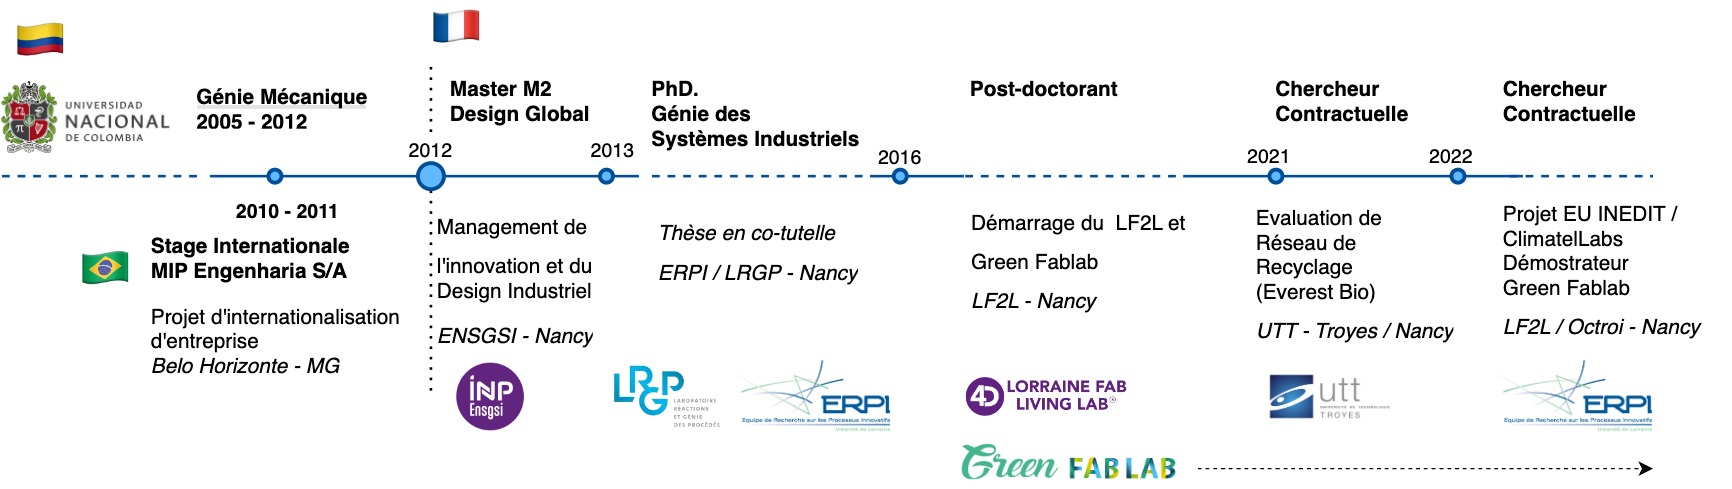
\includegraphics{Figures/slides/Fabio-timeline-Parcours.jpg}
\end{column}
\end{columns}

\note{}
\end{frame}

\hypertarget{activituxe9s-de-recherche}{%
\subsection{Activités de Recherche}\label{activituxe9s-de-recherche}}

\begin{frame}[t]{Thématique de Recherche}
\protect\hypertarget{thuxe9matique-de-recherche}{}
\small

Recyclage des thermoplastiques en circuit court par fabrication additive
open source.

\begin{figure}

{\centering 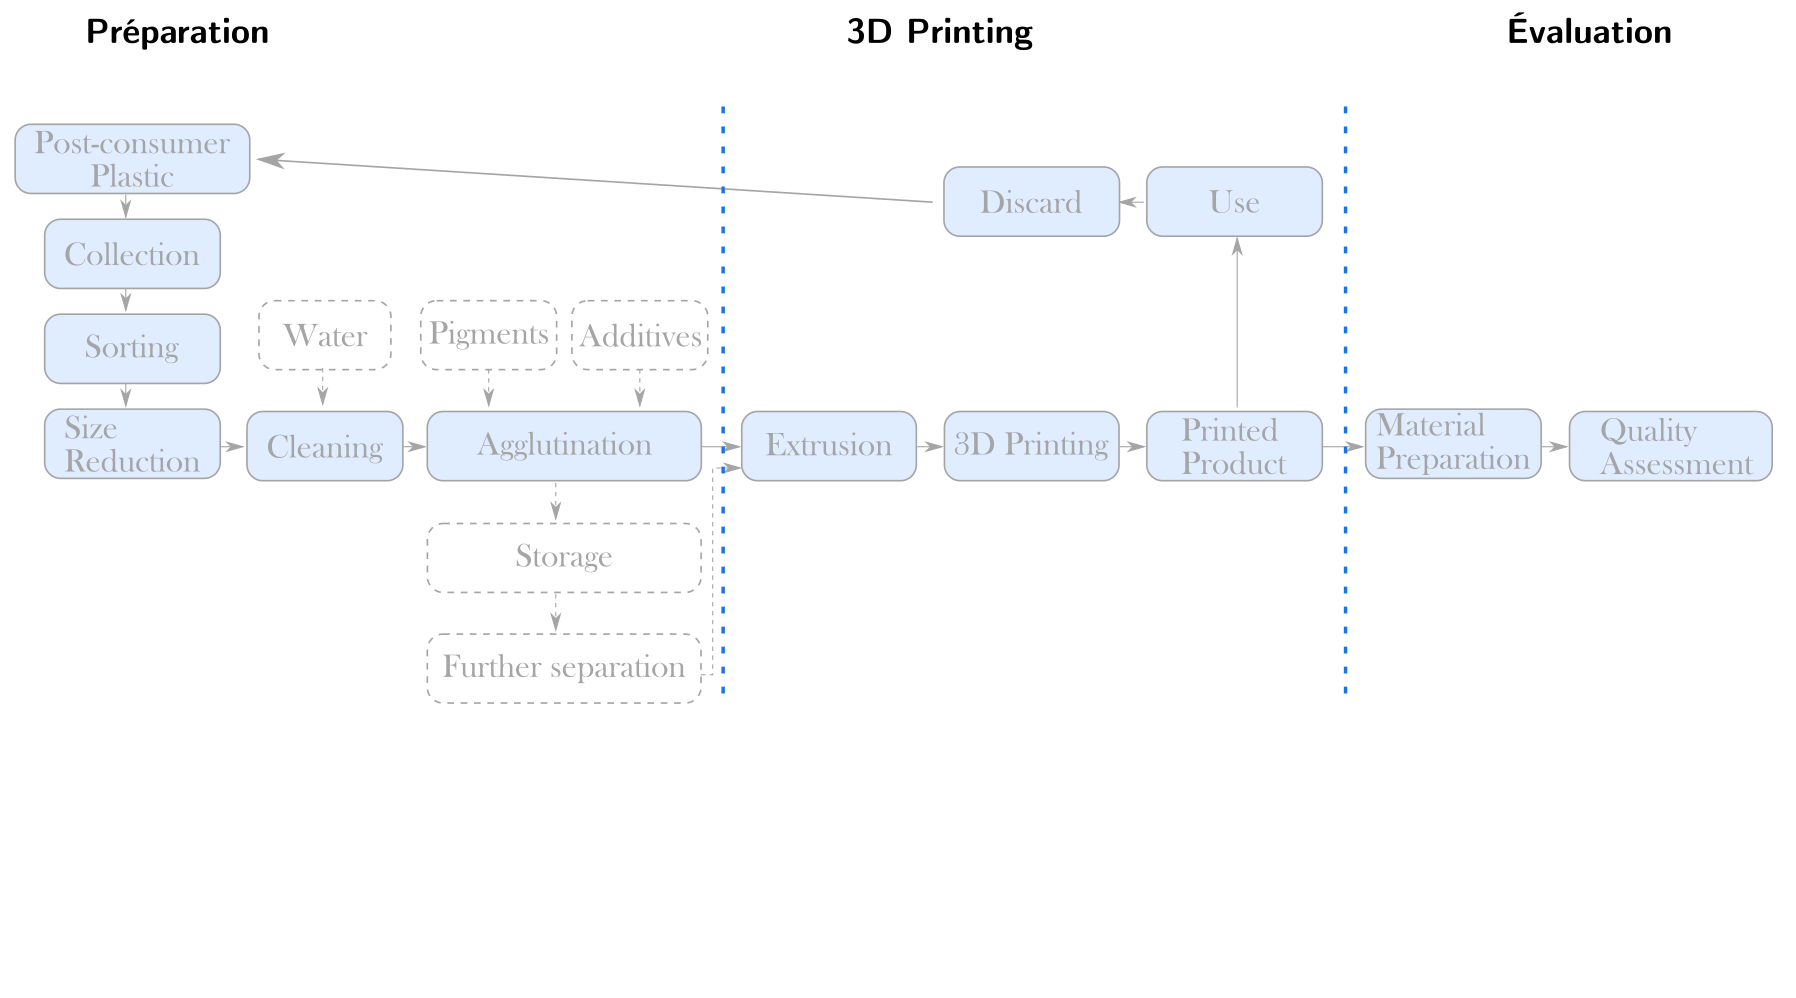
\includegraphics[width=0.75\textwidth,height=\textheight]{Figures/slides/DRAM-01.png}

}

\end{figure}

\note{}
\end{frame}

\begin{frame}[t]{Thématique de Recherche}
\protect\hypertarget{thuxe9matique-de-recherche-1}{}
\small

\textbf{Recyclage} des thermoplastiques en circuit court \textbf{par
fabrication additive open source}

\begin{figure}

{\centering 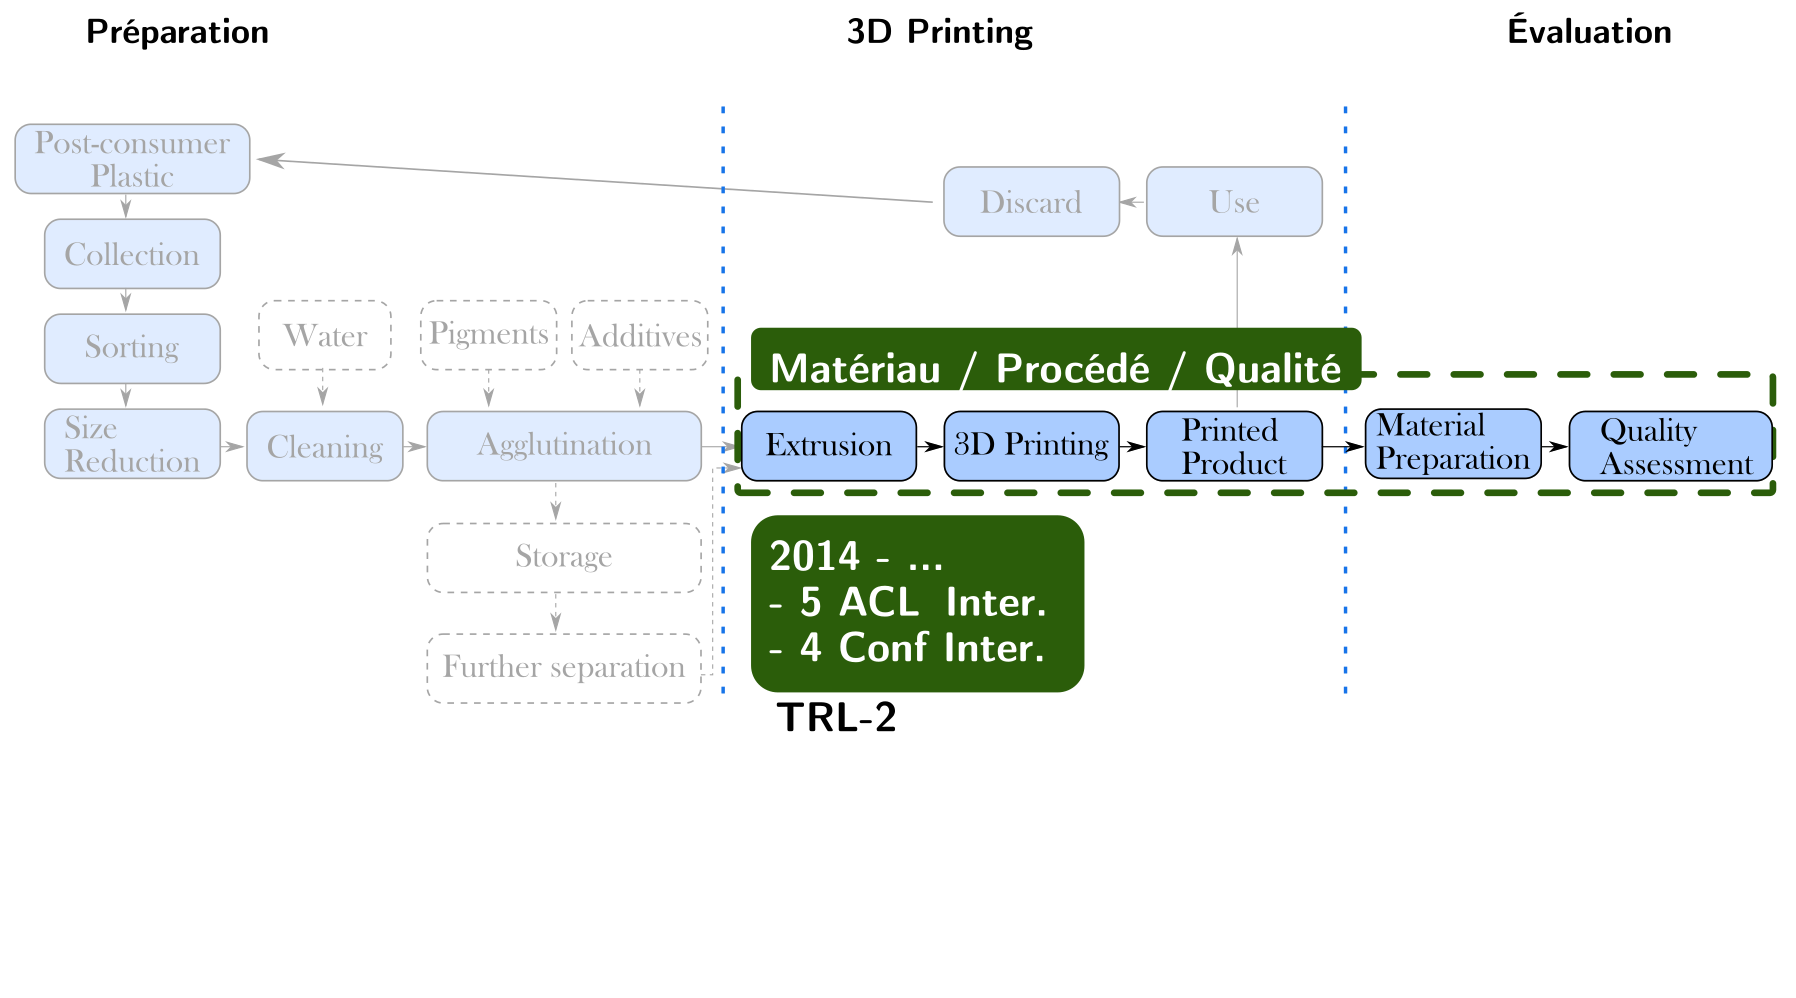
\includegraphics[width=0.75\textwidth,height=\textheight]{Figures/slides/DRAM-02.png}

}

\end{figure}
\end{frame}

\begin{frame}[t]{Thématique de Recherche}
\protect\hypertarget{thuxe9matique-de-recherche-2}{}
\small

\textbf{Recyclage} des thermoplastiques en \textbf{circuit court par
fabrication additive open source}

\begin{figure}

{\centering 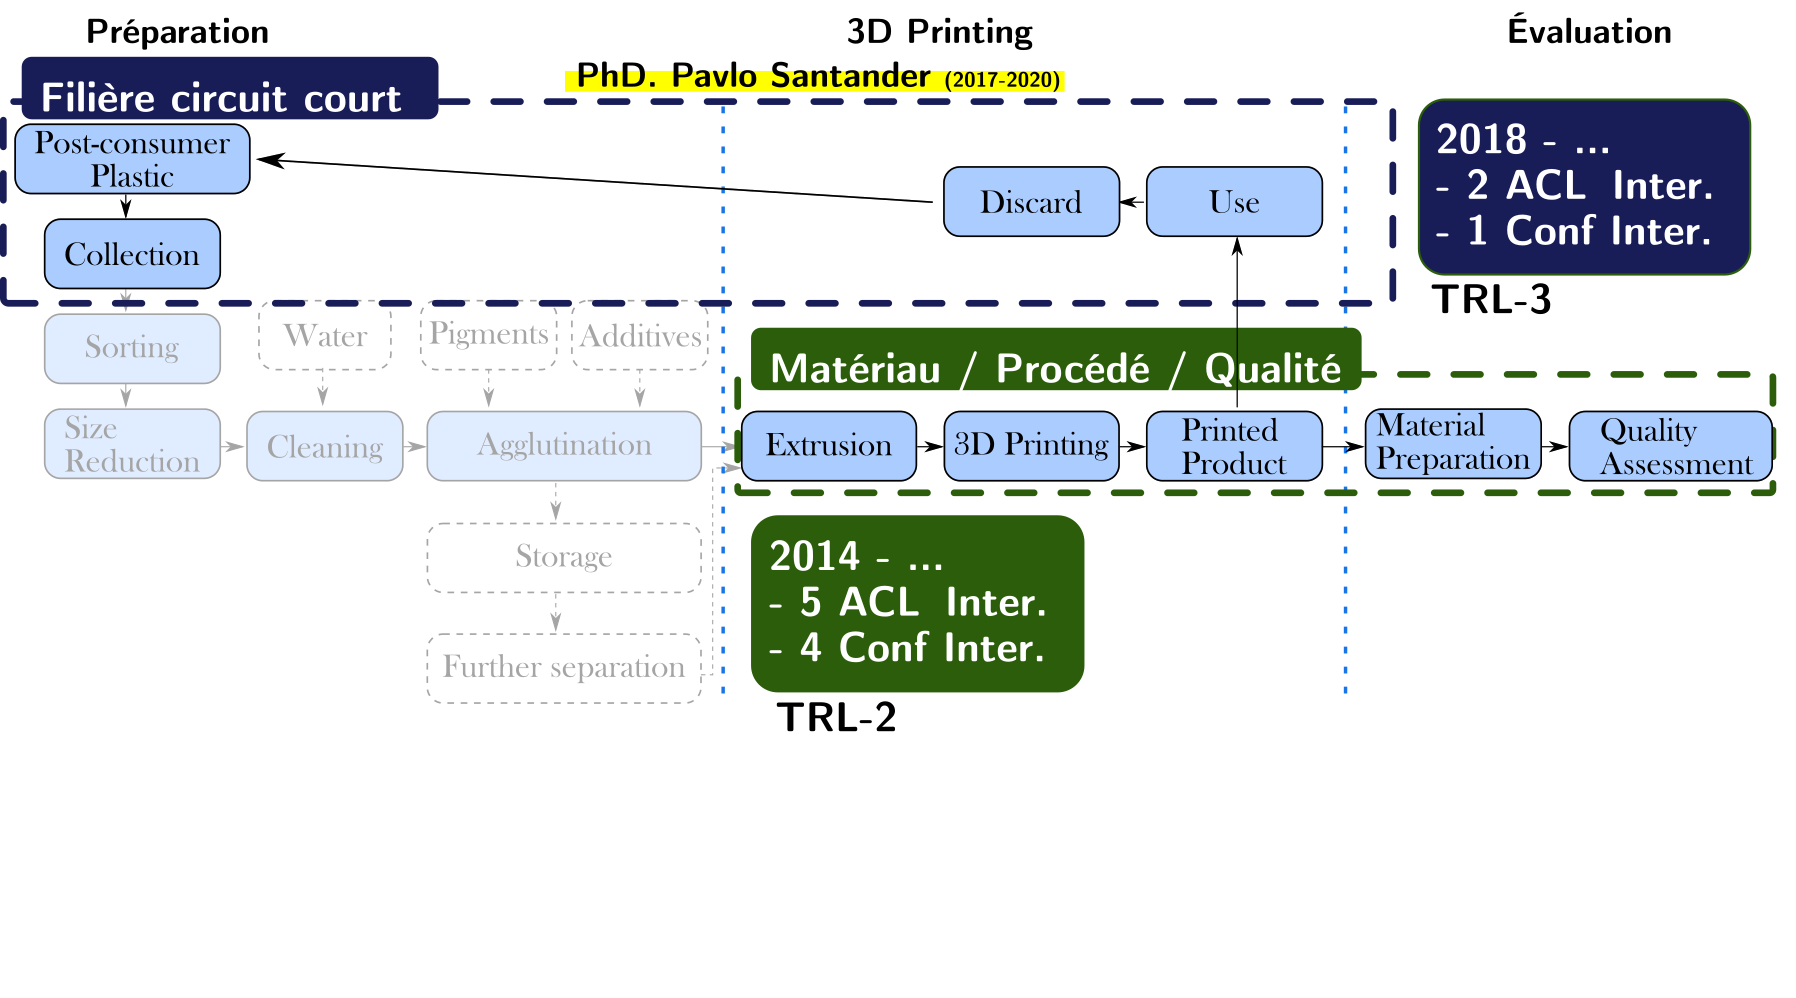
\includegraphics[width=0.75\textwidth,height=\textheight]{Figures/slides/DRAM-03.png}

}

\end{figure}
\end{frame}

\begin{frame}[t]{Thématique de Recherche}
\protect\hypertarget{thuxe9matique-de-recherche-3}{}
\small

\textbf{Recyclage des thermoplastiques en circuit court par fabrication
additive open source}

\begin{figure}

{\centering 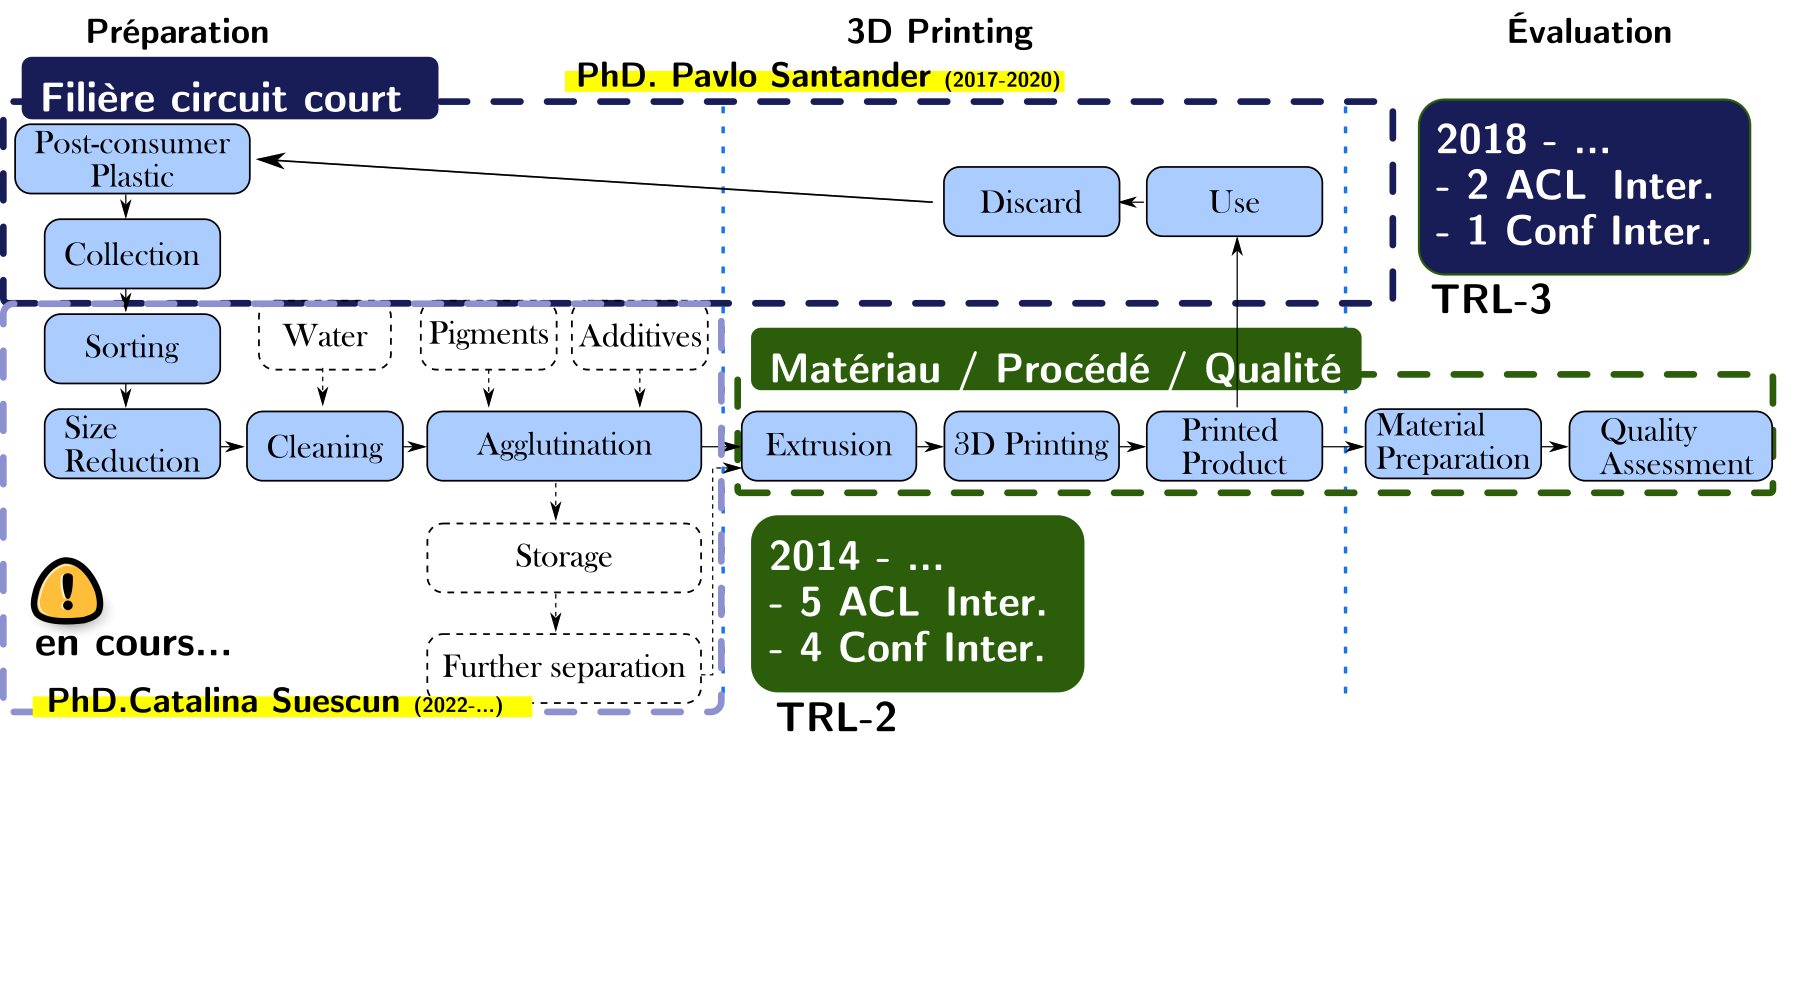
\includegraphics[width=0.75\textwidth,height=\textheight]{Figures/slides/DRAM-04.png}

}

\end{figure}
\end{frame}

\begin{frame}[t]{Thématique de Recherche}
\protect\hypertarget{thuxe9matique-de-recherche-4}{}
\small

\textbf{Recyclage des thermoplastiques en circuit court par fabrication
additive open source}

\begin{figure}

{\centering 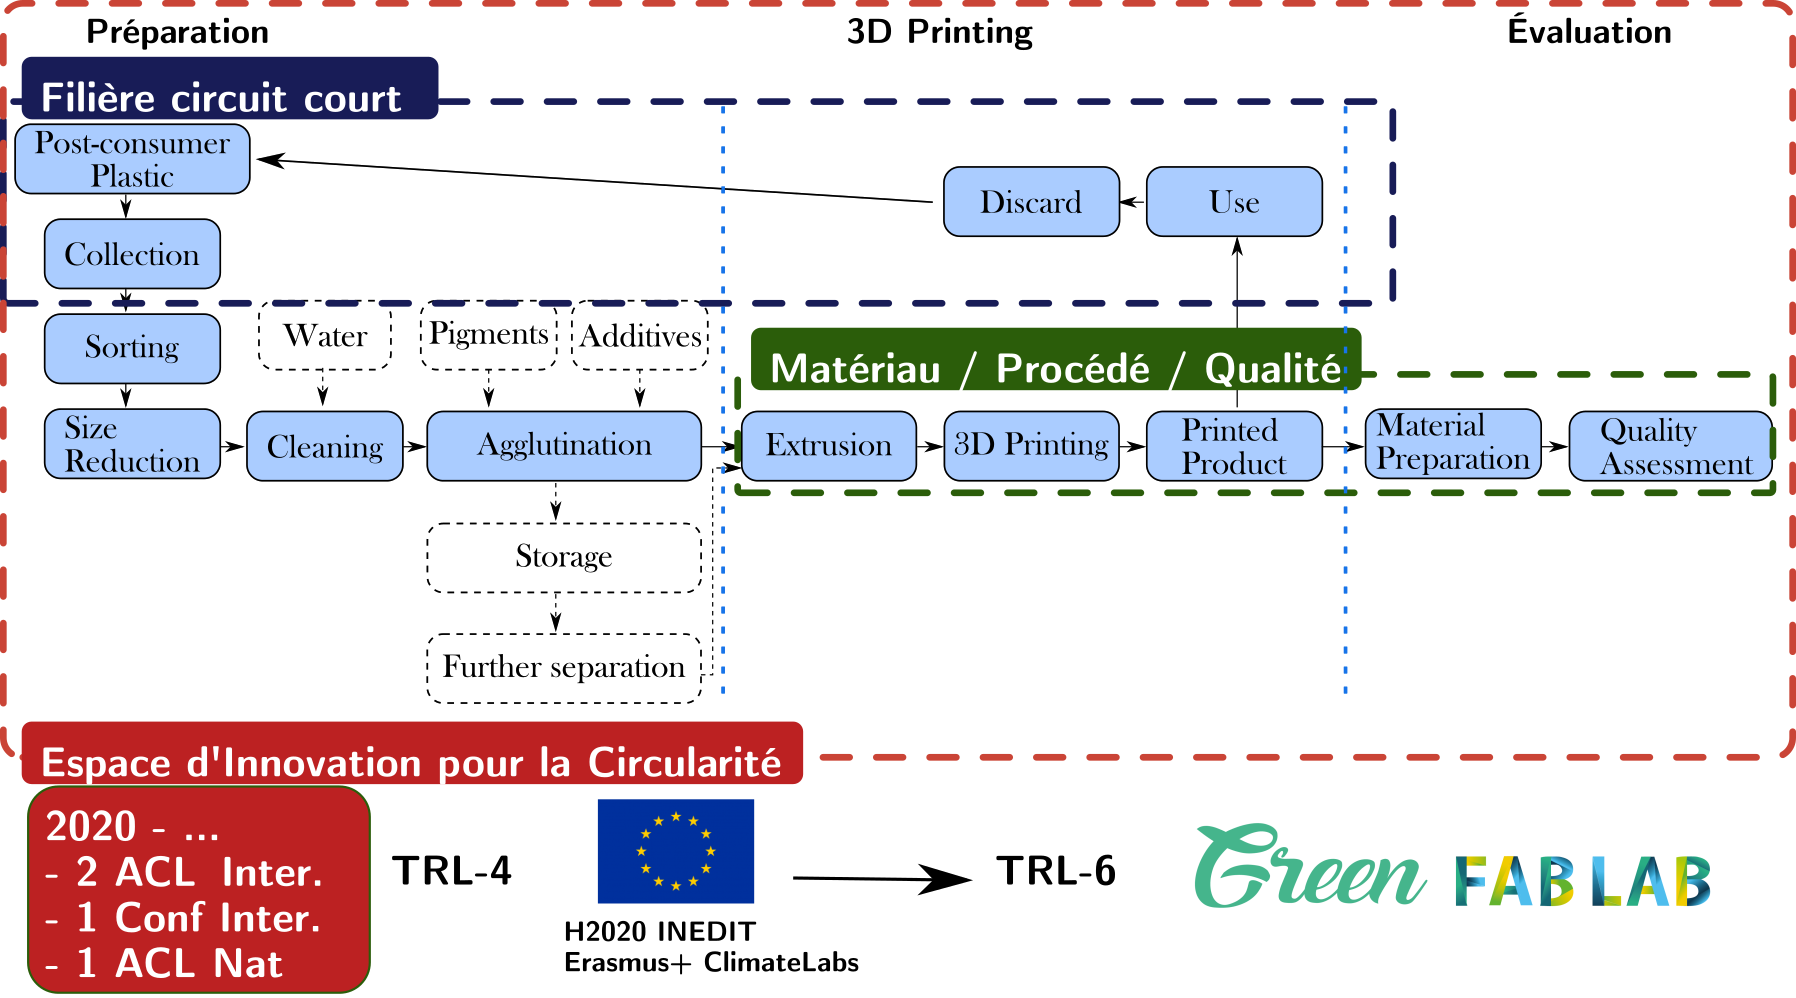
\includegraphics[width=0.75\textwidth,height=\textheight]{Figures/slides/DRAM-05.png}

}

\end{figure}
\end{frame}

\begin{frame}[t]{Thématique de Recherche}
\protect\hypertarget{thuxe9matique-de-recherche-5}{}
Recherche-action via un demonstrateur territorial en mode \emph{living
lab}.

\begin{figure}

{\centering 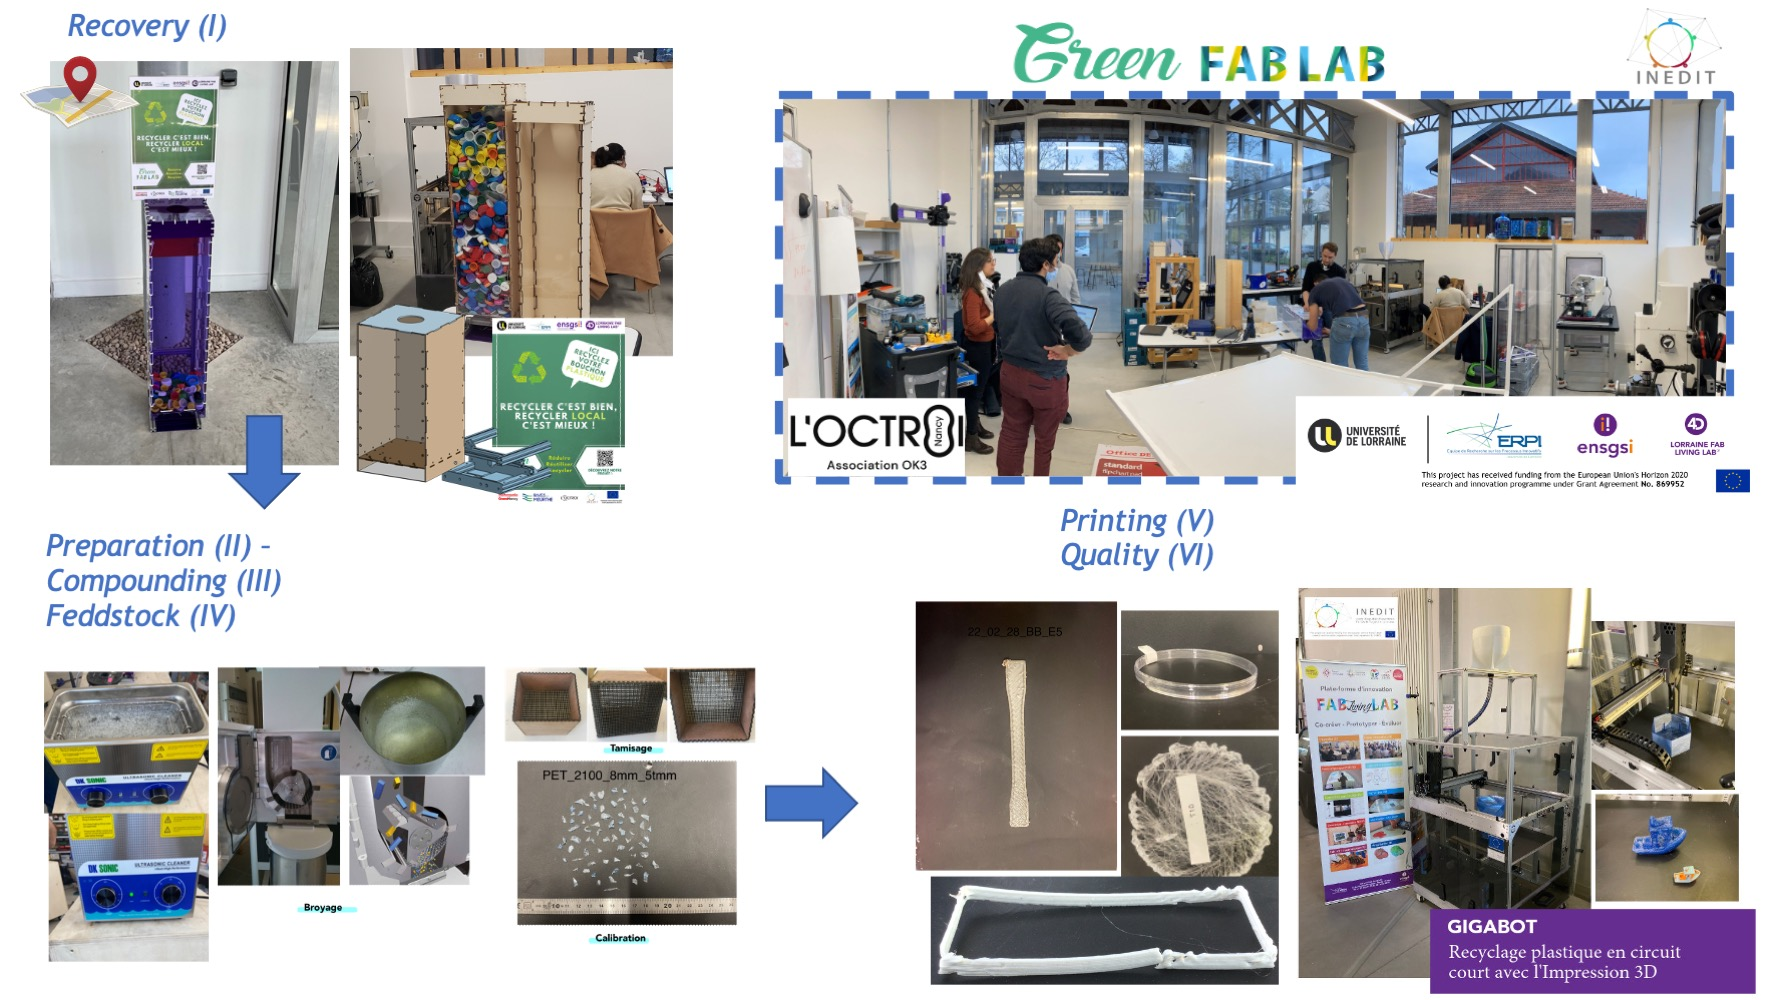
\includegraphics[width=0.7\textwidth,height=\textheight]{Figures/INEDIT.jpg}

}

\end{figure}
\end{frame}

\begin{frame}{Bilan Production Scientifique}
\protect\hypertarget{bilan-production-scientifique}{}
\begin{columns}[T]
\begin{column}[T]{0.5\textwidth}
\scriptsize

\textbf{Quantitatif:}

\begin{itemize}
\tightlist
\item
  9 articles ACL internationaux, 3 soumis\\
\item
  6 conférences internationales\\
\item
  2 Chapiters soumis.
\item
  2 conférences nationales
\end{itemize}
\end{column}

\begin{column}[T]{0.5\textwidth}
\scriptsize

\textbf{Scopus}:

\begin{columns}[T]
\begin{column}[T]{0.3\textwidth}
\scriptsize

\begin{itemize}
\tightlist
\item
  H6,
\item
  11 Docs
\item
  449 Cit.
\end{itemize}
\end{column}

\begin{column}[T]{0.7\textwidth}
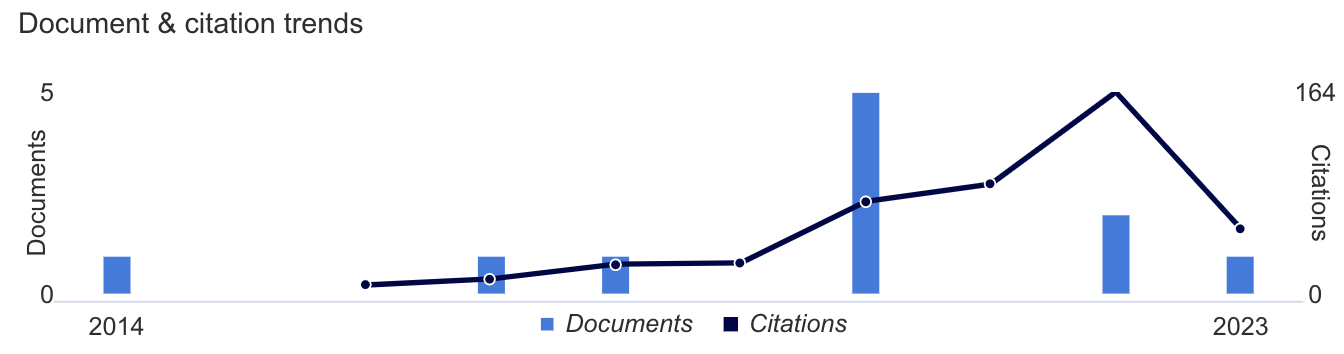
\includegraphics{Figures/slides/Scopus.png}
\end{column}
\end{columns}
\end{column}
\end{columns}

\pause

\scriptsize

\textbf{Qualitatif:}

\begin{figure}

{\centering 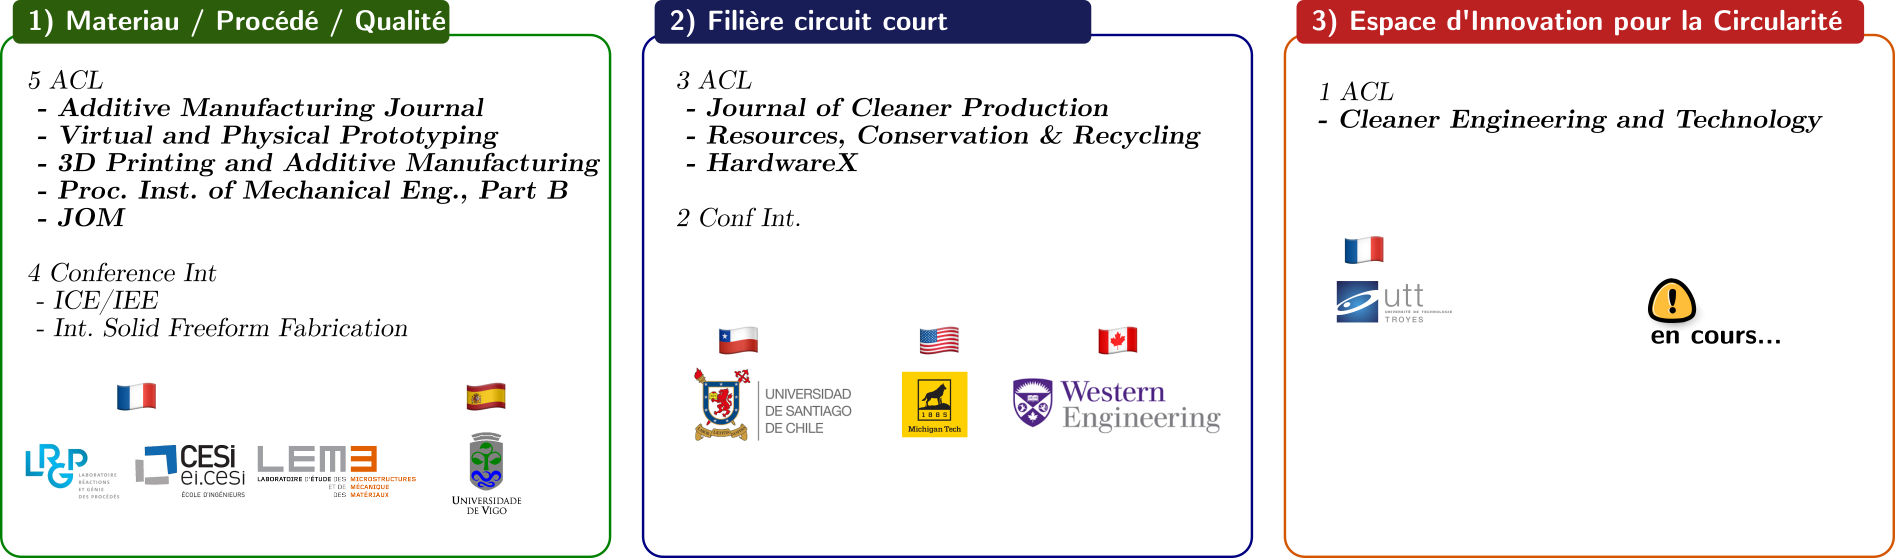
\includegraphics[width=0.8\textwidth,height=\textheight]{Figures/slides/Partners.png}

}

\end{figure}
\end{frame}

\begin{frame}{Participation au montage et à la redaction des projets}
\protect\hypertarget{participation-au-montage-et-uxe0-la-redaction-des-projets}{}
\begin{figure}

{\centering 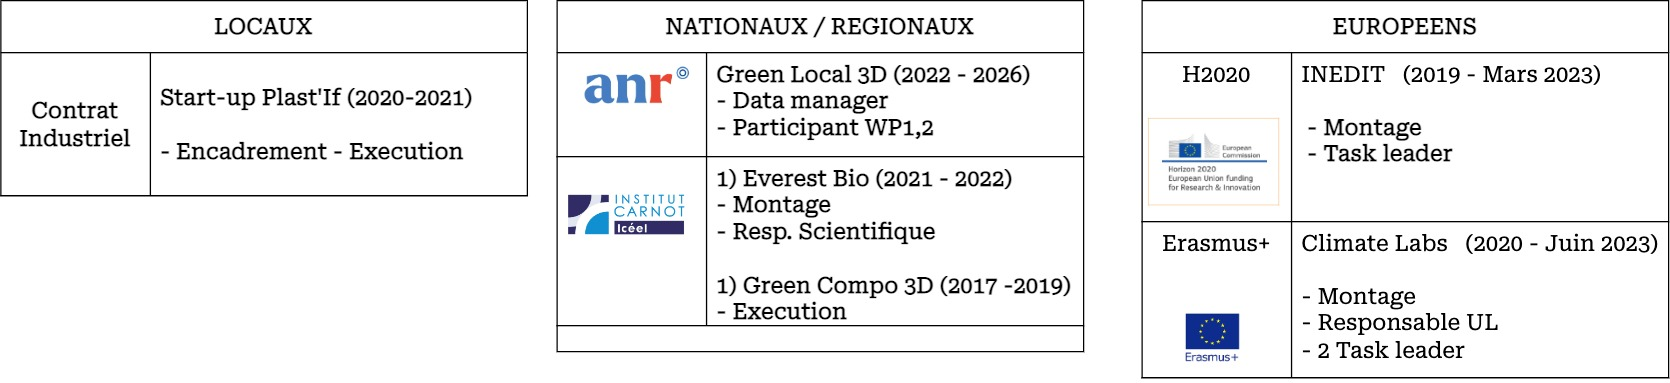
\includegraphics[width=0.9\textwidth,height=\textheight]{Figures/slides/Fabio-timeline-Projects.jpg}

}

\end{figure}
\end{frame}

\hypertarget{activituxe9s-denseignement}{%
\subsection{Activités d'Enseignement}\label{activituxe9s-denseignement}}

\begin{frame}{Synthèse des activités d'Enseignement}
\protect\hypertarget{synthuxe8se-des-activituxe9s-denseignement}{}
\begin{columns}[T]
\begin{column}[c]{0.5\textwidth}
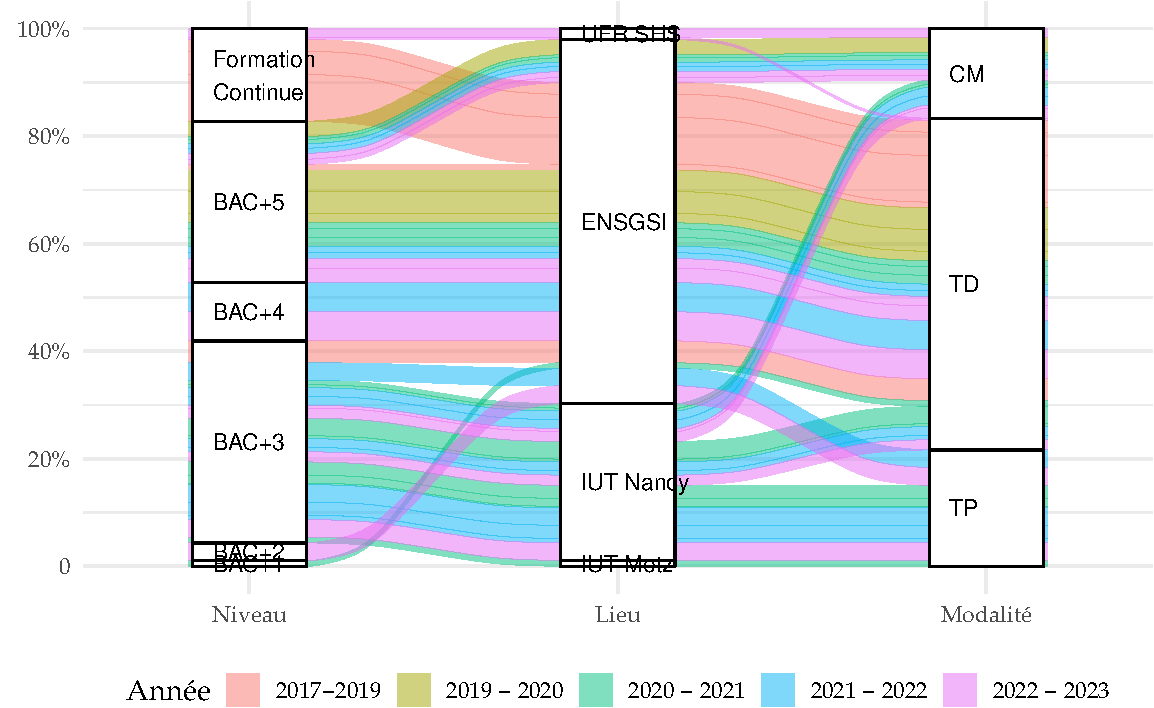
\includegraphics{figures/fig-sankey-1.pdf}
\end{column}

\begin{column}[c]{0.5\textwidth}
\small

\begin{itemize}
\item
  Enseignements depuis 2017 : \textbf{387 h}
\item
  \textbf{ENSGSI:} Pole Conception et Innovation

  \begin{itemize}
  \tightlist
  \item
    Module Recherche, Developpement et Innovation
  \end{itemize}
\item
  \textbf{IUT Charlemagne:} LP Animateur Facilitateur de Tiers-Lieux
  Éco-Responsables (AFTER)

  \begin{itemize}
  \tightlist
  \item
    Création de 2 modules
  \end{itemize}
\end{itemize}
\end{column}
\end{columns}
\end{frame}

\begin{frame}[t]{Module de Formation Mis en oeuvre}
\protect\hypertarget{module-de-formation-mis-en-oeuvre}{}
\textbf{CI15 Recherche, Developpement et Innovation} \hfill (2017 -
\ldots)

\begin{columns}[T]
\begin{column}[c]{0.5\textwidth}
\scriptsize

\begin{itemize}
\tightlist
\item
  Faire le lien entre la \textbf{démarche scientifique et leur sujet de
  stage!}, pour qu'ils deviennent force de proposition en s'appuyant sur
  la recherche.
\end{itemize}
\end{column}

\begin{column}[c]{0.5\textwidth}
\scriptsize

\begin{itemize}
\tightlist
\item
  Niveau BAC+5: ENSGSI 3AI, Master M2 IDEAS \& IUVTT
\end{itemize}
\end{column}
\end{columns}

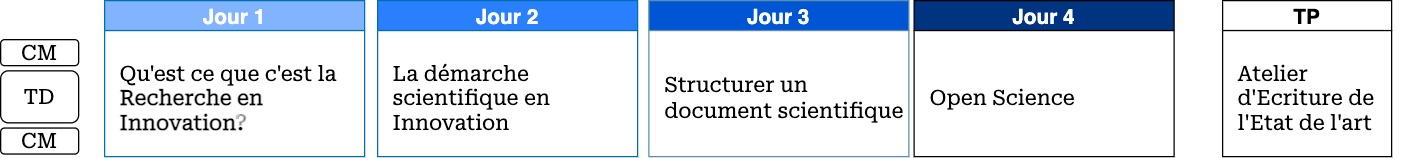
\includegraphics{figures/slides/Ensegnement-CI15.jpg}

\begin{columns}[T]
\begin{column}[T]{0.5\textwidth}
\footnotesize

\begin{itemize}
\tightlist
\item
  \textbf{Support Numérique Pédagogique}
\end{itemize}

\begin{figure}

{\centering 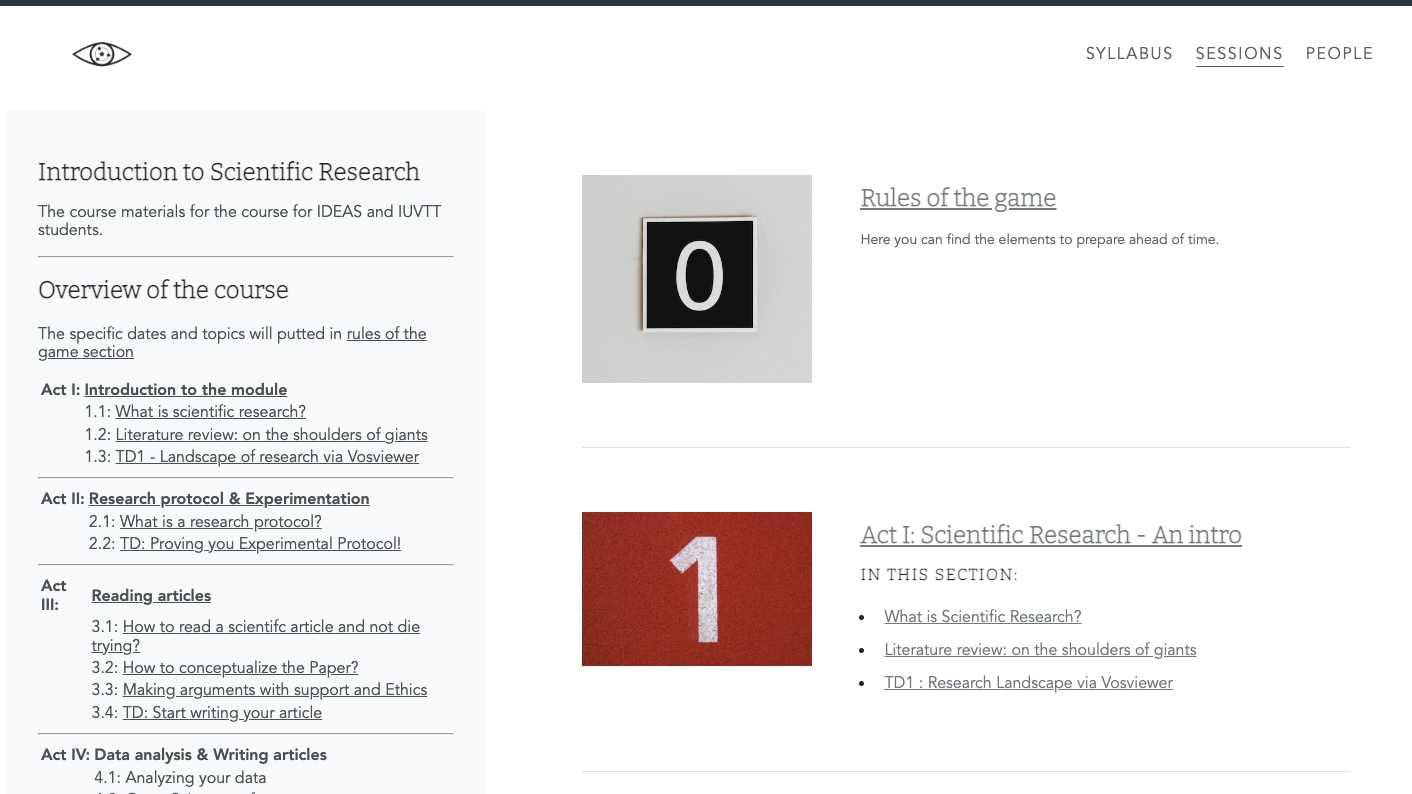
\includegraphics[width=1.04167in,height=\textheight]{figures/slides/CI15-web.png}

}

\end{figure}

https://ci15.netlify.app/
\end{column}

\begin{column}[T]{0.5\textwidth}
\footnotesize

\begin{itemize}
\tightlist
\item
  \textbf{Sciences de données \(\rightarrow\) Réproductibilité}
\end{itemize}

\begin{figure}

{\centering 
\includegraphics[width=1.25in,height=\textheight]{figures/slides/Rlogo.png}

}

\end{figure}
\end{column}
\end{columns}
\end{frame}

\begin{frame}{Recherche \(\rightarrow\) Pédagogie: Modules LP AFTER}
\protect\hypertarget{recherche-rightarrow-puxe9dagogie-modules-lp-after}{}
\scriptsize

\begin{itemize}
\tightlist
\item
  Maîtriser et s'approprier les notions clés du recyclage
\item
  Impliquer les étudiants dans une démarche de construction pédagogique
\end{itemize}

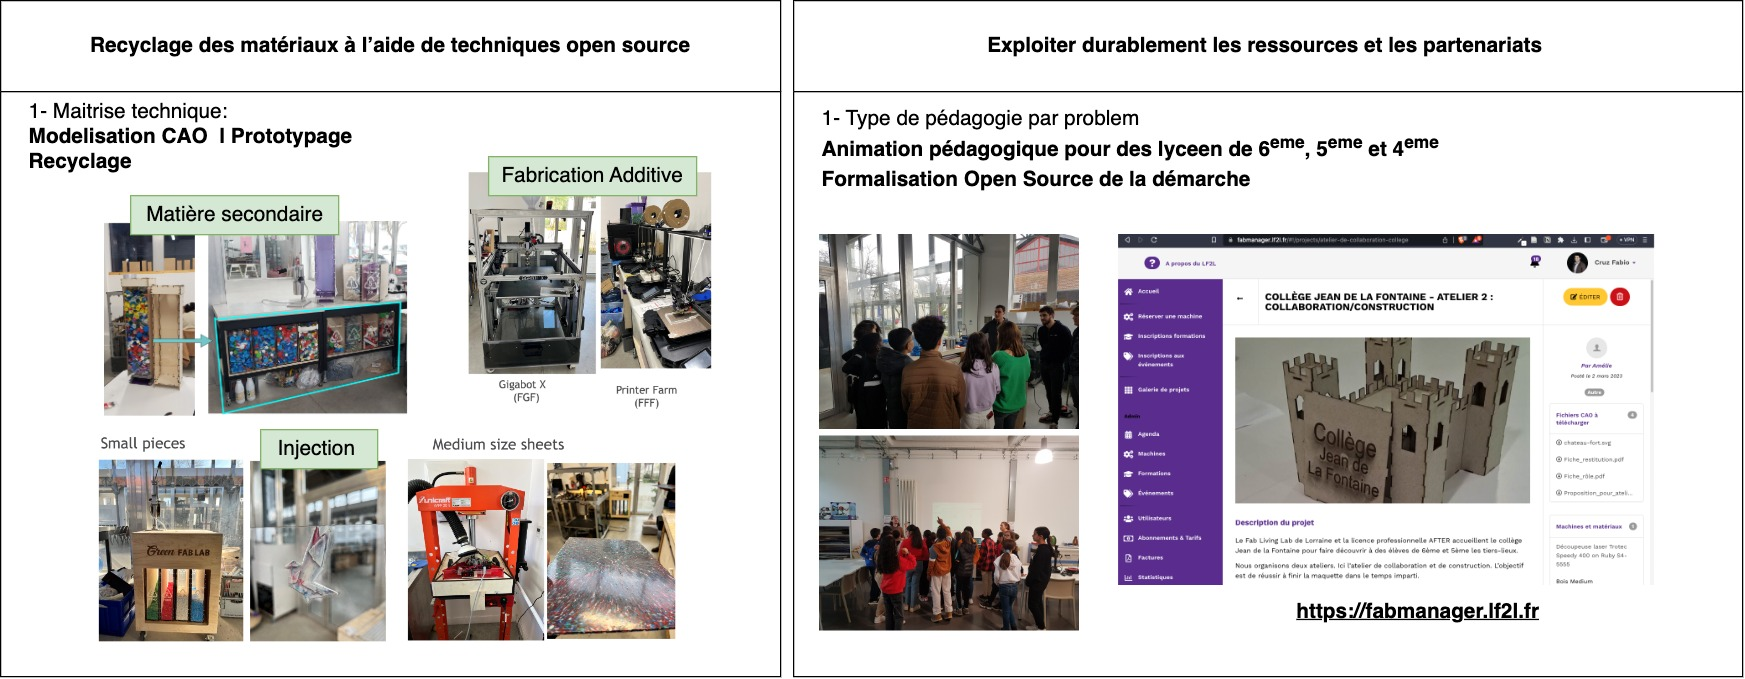
\includegraphics[width=0.9\textwidth,height=\textheight]{figures/slides/Ensegnement-AFTER.jpg}

\normalsize
\end{frame}

\hypertarget{responsabilituxe9s-collectives-et-valorisation}{%
\subsection{responsabilités collectives et
Valorisation}\label{responsabilituxe9s-collectives-et-valorisation}}

\begin{frame}{responsabilités collectives et Valorisation}
\begin{block}{Vie du Laboratoire}
\protect\hypertarget{vie-du-laboratoire}{}
\scriptsize

\begin{itemize}
\tightlist
\item
  Support au LF2L \textbar{} Labelisation
\item
  GT Numerique
\item
  Montage de projets de recherche (EU, Nationaux)
\item
  Reseaux: GRD MACS - Soutenabilité \textbar{} DfAM (UK)
\end{itemize}
\end{block}

\begin{block}{Vie de l'Ecole}
\protect\hypertarget{vie-de-lecole}{}
\scriptsize

\begin{itemize}
\tightlist
\item
  Animation de séances de prototypage
\item
  Journées Portes Ouvertes
\item
  `Coup de Coeur' de \textbf{Trophées francophones des Campus
  Responsables 2023} - Utopies - Min. Trans. Ecol / Ens. Sup. et Rech.
\end{itemize}
\end{block}

\begin{block}{Vulgarisation scientifique}
\protect\hypertarget{vulgarisation-scientifique}{}
\scriptsize

\begin{itemize}
\tightlist
\item
  Gagnant à la finale régionale de «\emph{Ma thèse en 180 secondes}»
\item
  Foire internationale de Nancy - Green Fablab depuis 2018
\item
  Conferences grand public au LF2L
\end{itemize}
\end{block}
\end{frame}

\hypertarget{proposition-dintuxe9gration}{%
\section{Proposition d'intégration}\label{proposition-dintuxe9gration}}

\hypertarget{lensgsi-et-lerpi}{%
\subsection{l'ENSGSI et l'ERPI}\label{lensgsi-et-lerpi}}

\begin{frame}[t]{l'ENSGSI et l'ERPI}
\begin{columns}[T]
\begin{column}[T]{0.5\textwidth}
Ma proposition pour l'ENSGSI: \vspace{1cm}

\textbf{Génie de l'Innovation Soutenable et Responsable}
\end{column}

\begin{column}[T]{0.5\textwidth}
Ma proposition pour l'ERPI:

\vspace{1cm}

\textbf{Mieux comprendre les systèmes socio-techniques de recyclage
distribuée en milieu urbain supportes par l'Open hardware}

\vfill
\end{column}
\end{columns}

\large

\normalsize
\end{frame}

\hypertarget{projet-de-recherche}{%
\subsection{Projet de Recherche}\label{projet-de-recherche}}

\begin{frame}[t]{Projet de Recherche}
\begin{columns}[T]
\begin{column}{0.6\textwidth}
\begin{figure}

{\centering 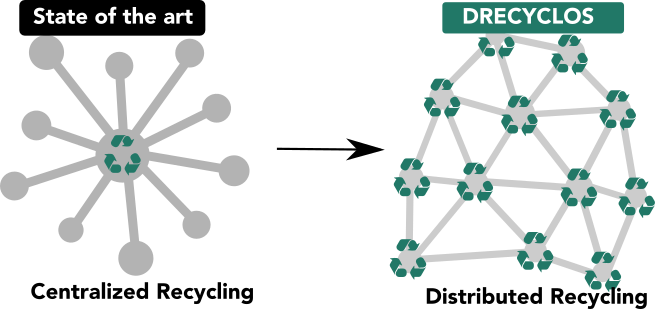
\includegraphics[width=0.8\textwidth,height=\textheight]{Figures/slides/ERC.png}

}

\end{figure}
\end{column}

\begin{column}{0.4\textwidth}
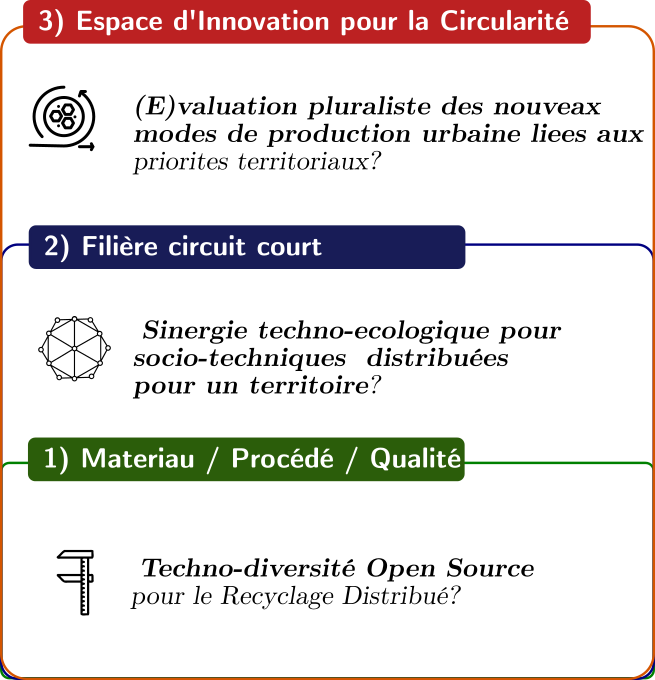
\includegraphics{Figures/slides/Projet-ERPI.png}
\end{column}
\end{columns}

\note{\begin{itemize}
\item
  Thèmes de recherche:

  \begin{itemize}
  \tightlist
  \item
    Aide à la conception en amont
  \item
    Acceptabilité du produit, du processus et de la filière
  \end{itemize}
\item
  Nouveaux démonstrateurs et protocoles expérimentaux Open Source
\item
  Recherche fondamental vers Recherche-action en mode Living Lab
\item
  (E)valuation Multi-acteurs et Multi-echelle
\end{itemize}}
\end{frame}

\begin{frame}[t]{Projet de Recherche}
\protect\hypertarget{projet-de-recherche-1}{}
\begin{columns}[T]
\begin{column}{0.6\textwidth}
\begin{figure}

{\centering 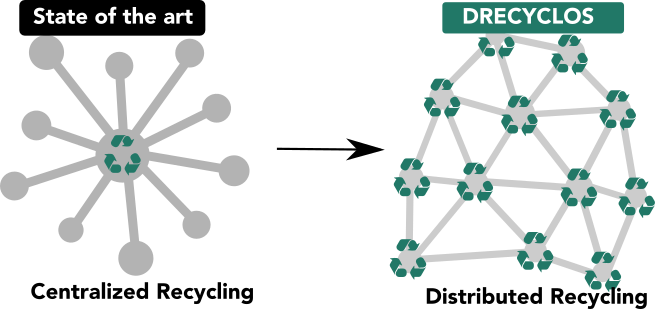
\includegraphics[width=0.8\textwidth,height=\textheight]{Figures/slides/ERC.png}

}

\end{figure}

\footnotesize

\begin{itemize}
\tightlist
\item
  Plastiques

  \begin{itemize}
  \tightlist
  \item
    Projet ANR `Green Local 3D' - 2022-2026 \textbar{} k€ 476
  \end{itemize}
\item
  WEEE

  \begin{itemize}
  \tightlist
  \item
    Projet LUE WEEEMET - 2022-2024 \textbar{} k€ 149
  \end{itemize}
\end{itemize}
\end{column}

\begin{column}{0.4\textwidth}
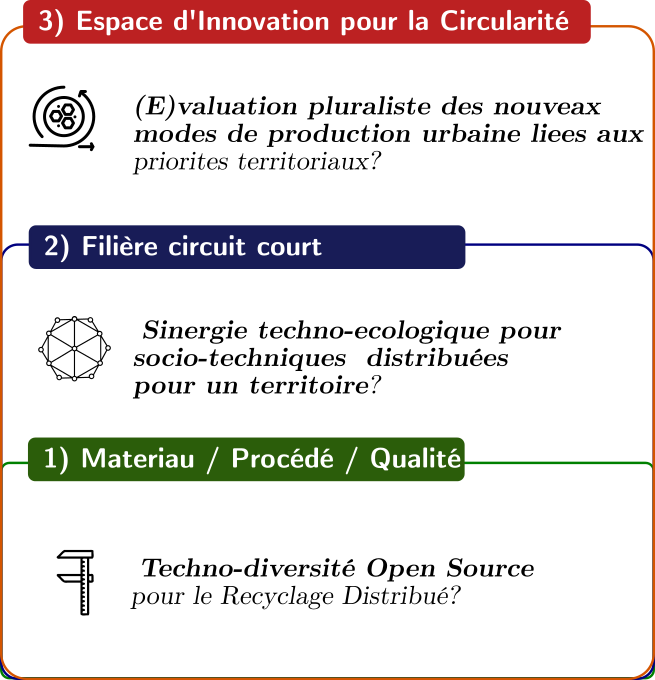
\includegraphics{Figures/slides/Projet-ERPI.png}
\end{column}
\end{columns}
\end{frame}

\hypertarget{projet-pedagogique}{%
\subsection{Projet Pedagogique}\label{projet-pedagogique}}

\begin{frame}{Ma vision de la pédagogique}
\protect\hypertarget{ma-vision-de-la-puxe9dagogique}{}
Développer des les conditions pour que l'élève :

\begin{itemize}
\item
  S'approprie et matérialise les connaissances en faisant par lui-même.
\item
  Développer des situations pédagogiques en mode \emph{agile} et
  \emph{active} en lien avec l'Open hardware et des communautés
  externes.
\item
  Faire le lien entre les enjeux sociétaux du développement durable et
  le parcours Ingénieur au niveau de la formation et de l'intégration
  professionnelle.
\end{itemize}
\end{frame}

\begin{frame}{Proposition d'Integration}
\protect\hypertarget{proposition-dintegration}{}
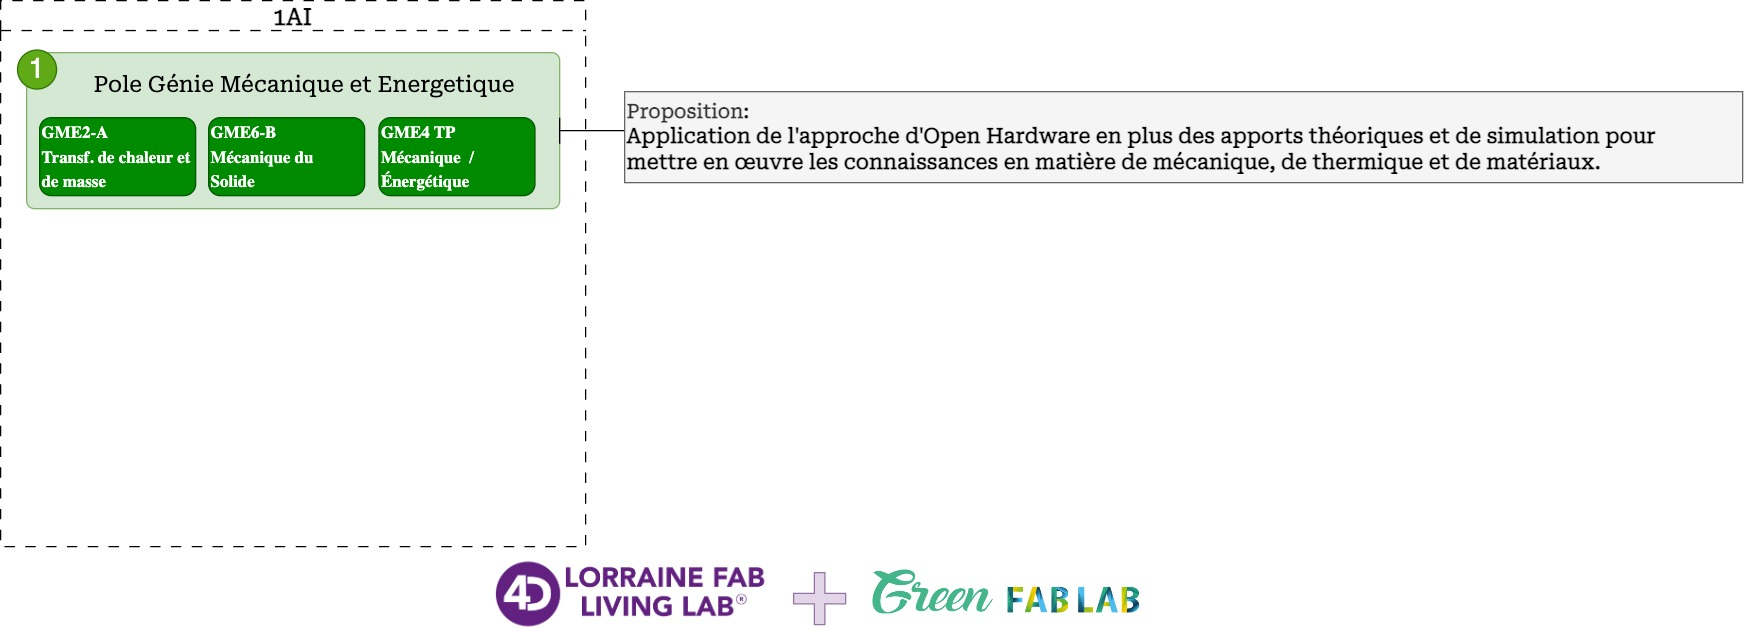
\includegraphics{Figures/slides/Ensegnement-Integration-01.jpg}
\end{frame}

\begin{frame}{Proposition d'Integration}
\protect\hypertarget{proposition-dintegration-1}{}
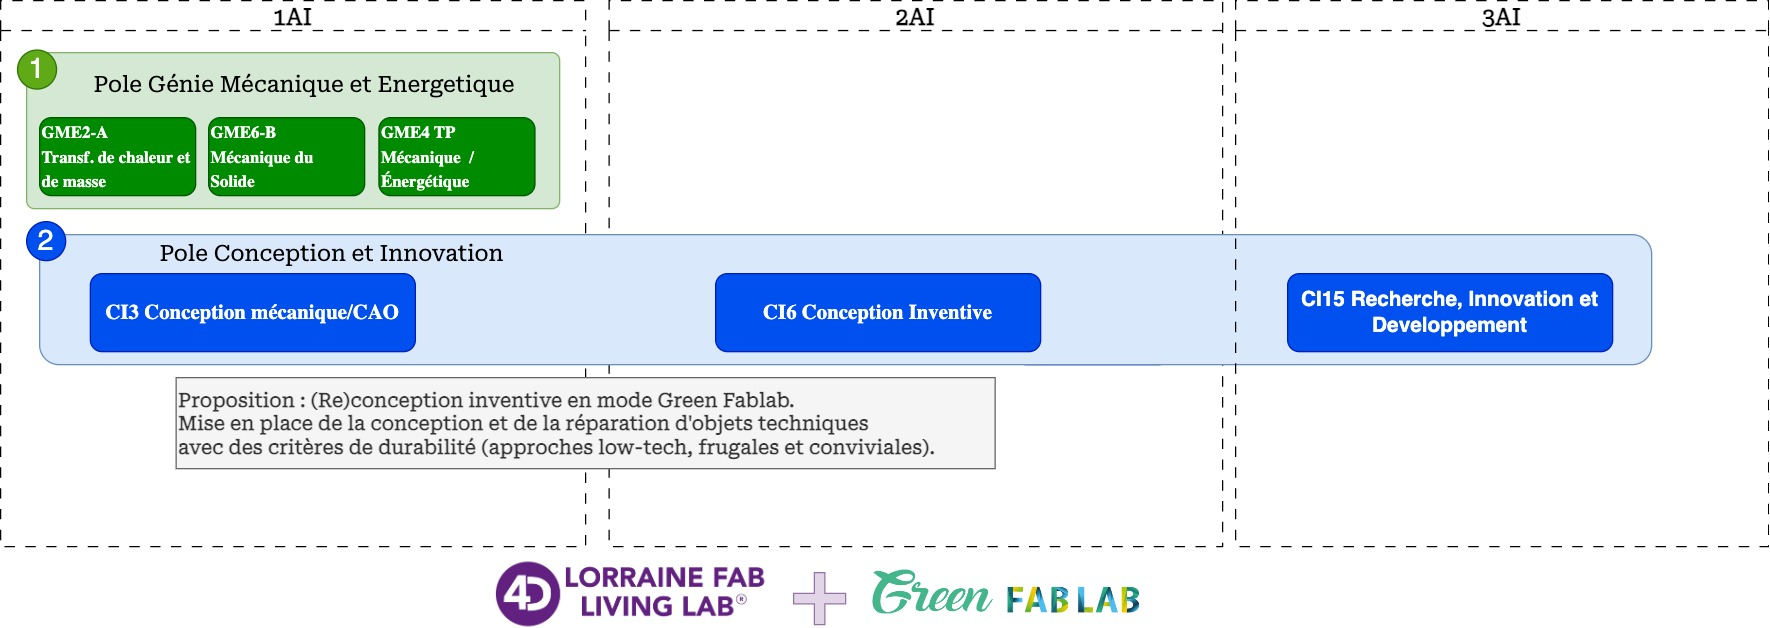
\includegraphics{Figures/slides/Ensegnement-Integration-02.jpg}
\end{frame}

\begin{frame}{Proposition d'Integration}
\protect\hypertarget{proposition-dintegration-2}{}
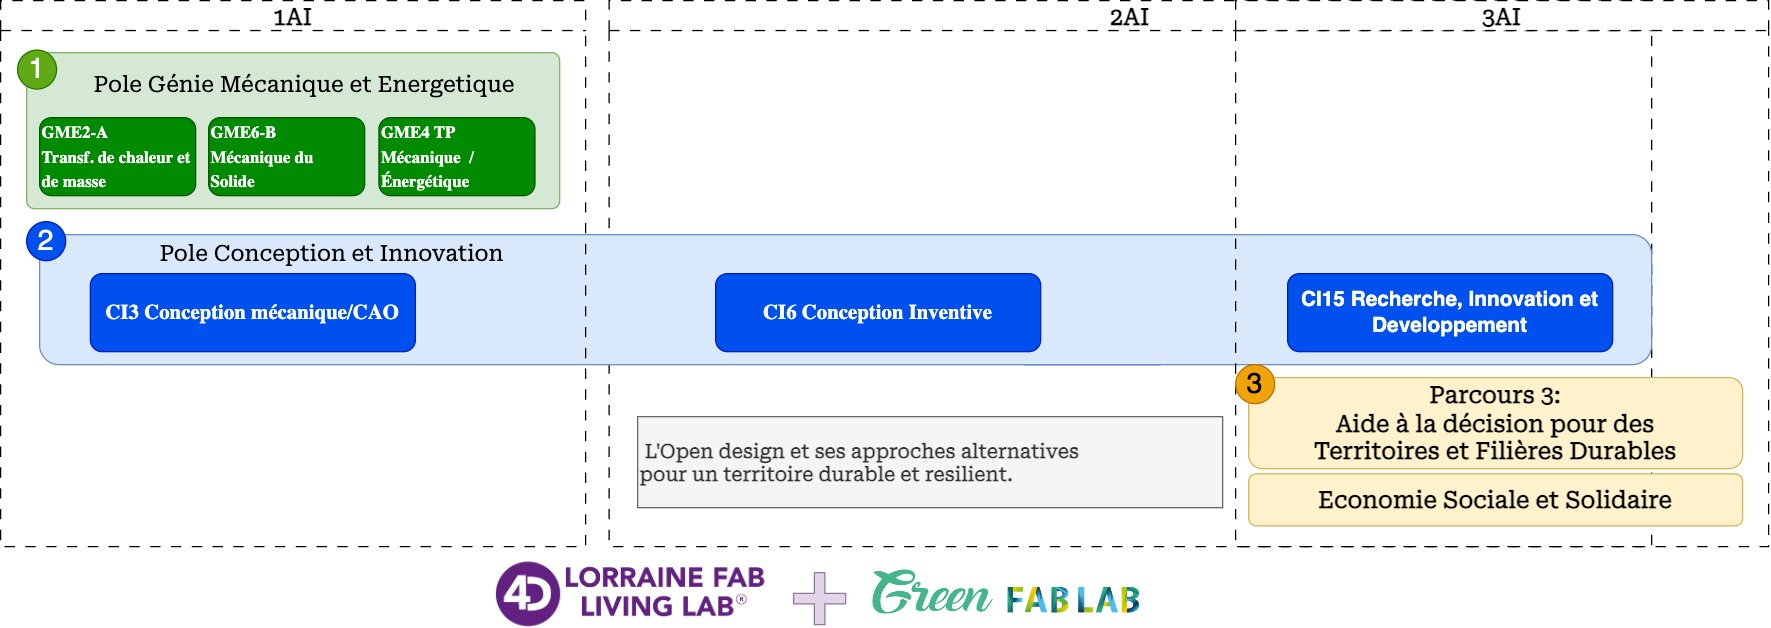
\includegraphics{Figures/slides/Ensegnement-Integration-03.jpg}

REC:

\begin{itemize}
\tightlist
\item
  \textbf{C7}: Promouvoir et mettre en oeuvre les principes de
  développement durable et de la responsabilité sociétale
\end{itemize}
\end{frame}

\hypertarget{conclusion}{%
\section{Conclusion}\label{conclusion}}

\begin{frame}{Conclusion}
Mon apport pour :

\begin{itemize}
\item
  \textbf{la Recherche}

  \begin{itemize}
  \tightlist
  \item
    Apporter mes competences pour une plus grande compréhension des
    \textbf{leviers socio-techniques} vers la soutenabilité de
    l'industrie.
  \end{itemize}
\item
  \textbf{la Pédagogie}

  \begin{itemize}
  \tightlist
  \item
    Valoriser la connaissance scientifique au travers de
    l'expérimentation au service du développement durable par
    l'Innovation.
  \end{itemize}
\item
  \textbf{le Collectif}

  \begin{itemize}
  \tightlist
  \item
    Participer aux projets industriels et pédagogiques, la vie de
    l'école et du laboratoire.
  \end{itemize}
\end{itemize}
\end{frame}

\begin{frame}{Merci beaucoup de votre attention}
\protect\hypertarget{merci-beaucoup-de-votre-attention}{}
\begin{block}{A disposition pour vos questions.}
\protect\hypertarget{a-disposition-pour-vos-questions.}{}
\end{block}
\end{frame}

\begin{frame}{Example en cours: TP Age du Faire et du DIY \hfill 2AP
ENSGSI}
\protect\hypertarget{example-en-cours-tp-age-du-faire-et-du-diy-2ap-ensgsi}{}
Transfer projeT EU H2020 INEDIT - Dec 2022.

\begin{columns}[T]
\begin{column}{0.6\textwidth}
\textbf{Idéation via VR:}

\begin{figure}

{\centering 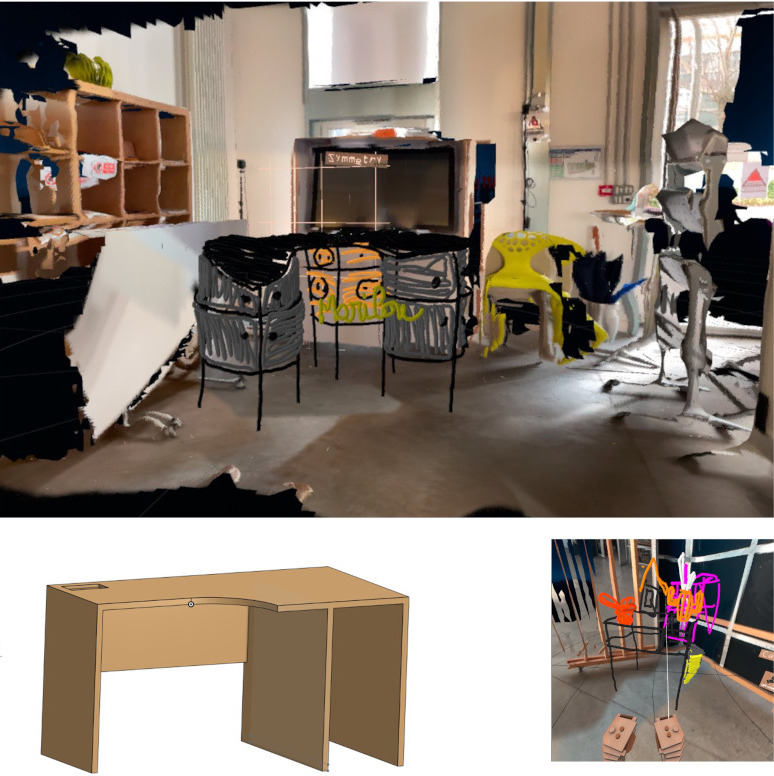
\includegraphics[width=0.5\textwidth,height=\textheight]{Figures/slides/Age-faire.jpg}

}

\end{figure}
\end{column}

\begin{column}{0.4\textwidth}
\textbf{Matérialisation récyclé:}

\begin{figure}

{\centering 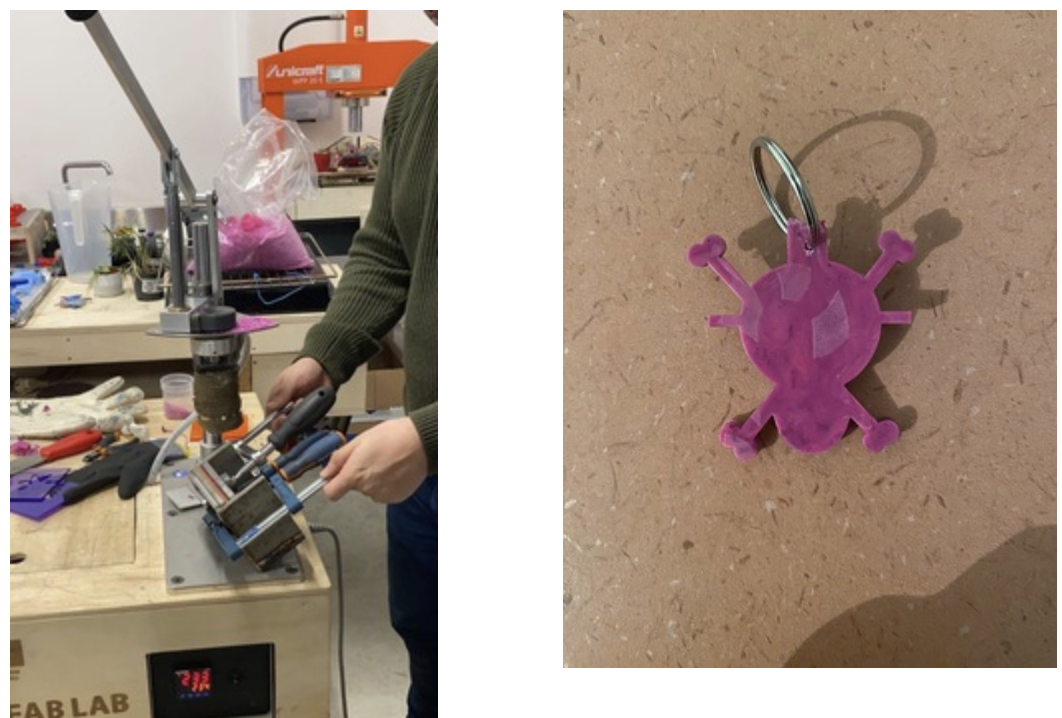
\includegraphics[width=1\textwidth,height=\textheight]{Figures/slides/Age-faire-1.png}

}

\end{figure}
\end{column}
\end{columns}
\end{frame}



\end{document}
